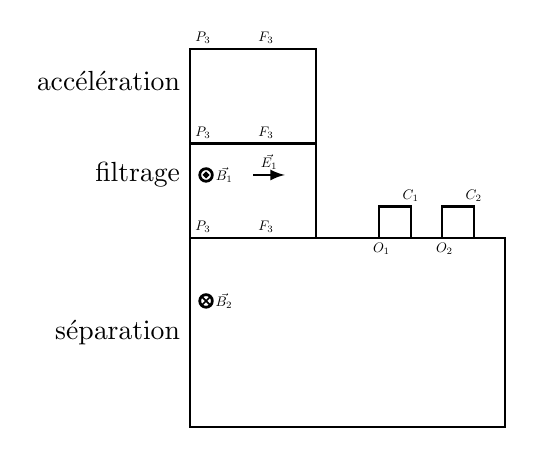
\begin{tikzpicture}[thick,scale=0.4, every node/.style={scale=0.5}]
	\draw (0,0) rectangle (10,6);
	\draw (6,6) rectangle ++(1,1) node[above]{$C_1$};
	
	\draw (6.5,6) node[below left]{$O_1$}
  node[color=white]{$\blacksquare$};
	\draw (8,6) rectangle ++(1,1)node[above]{$C_2$};
	\draw (8.5,6) node[below left]{$O_2$}
  node[color=white]{$\blacksquare$};
	\draw (0,6) node[above right]{$P_3$} -- ++(4,0) 
				node[midway,above right]{$F_3$} 
				node[midway,color=white]{$\blacksquare$};
	\draw (0,6)--(0,9) 
				node[above right]{$P_3$} -- ++(4,0) 
				node[midway,above right]{$F_3$} 
				node[midway,color=white]{$\blacksquare$} -- ++(0,-3);
	\draw (0,9)--(0,12) 
				node[above right]{$P_3$} -- ++(4,0) 
				node[midway,above right]{$F_3$} 
				node[midway,color=white]{$\blacksquare$} -- ++(0,-3);
	\filldraw[fill=white,line width=1pt](.5,4)circle(.2cm);
	\draw[line width=.6pt] (.5,4) node[right]{$~\vec{B_2}$}
	+(-135:.2cm) -- +(45:.2cm)
	+(-45:.2cm) -- +(135:.2cm);
	\filldraw[fill=white,line width=1pt](.5,8)circle(.2cm);
	\filldraw[fill=black,line width=1pt](.5,8)circle(.05cm) node[right]{$~\vec{B_1}$};
	\draw[>=latex,->] (2,8) -- (3,8) 		
						node[midway,above]{$\vec{E_1}$};
	\node[scale=2,left] at(0,3){séparation};
	\node[scale=2,left] at(0,8){filtrage};
	\node[scale=2,left] at(0,11){accélération};
\end{tikzpicture}